%!TEX root = ../hbrs-poster.tex


    \block{Methodology}
    {
        \textbf{Our approach involved the following steps:}
        \begin{enumerate}
            \item \textbf{Data Acquisition and Cleaning:} Loading and inspecting the dataset from Kaggle \cite{kaggle_toxic}. Applying preprocessing steps such as lowercasing, punctuation removal, and tokenization. Handling missing data and analyzing class imbalance.
            \item \textbf{Embeddings:} Integrating various word embeddings (e.g., pretrained GloVe, FastText) and evaluating their effect on model performance.
            \item \textbf{Model Training:} Implementing and comparing several neural network architectures:
                \begin{itemize}
                    \item Simple RNN, LSTM, GRU, BiLSTM.
                    \item Transformer encoder (e.g., DistilBERT or BERT fine-tuning).
                    \item Finetuning LLMs like GPT-1 and Llama 3.2 using LoRA.
                \end{itemize}
            \item \textbf{Threshold Optimization:} Use validation data to tune thresholds for each label instead of defaulting to 0.5, which may not be optimal due to class imbalance.
            \item \textbf{Evaluation:} Evaluate using standard metrics (e.g., ROC-AUC, F1-score) and analyze per-class performance.
        \end{enumerate}

        \begin{center}
            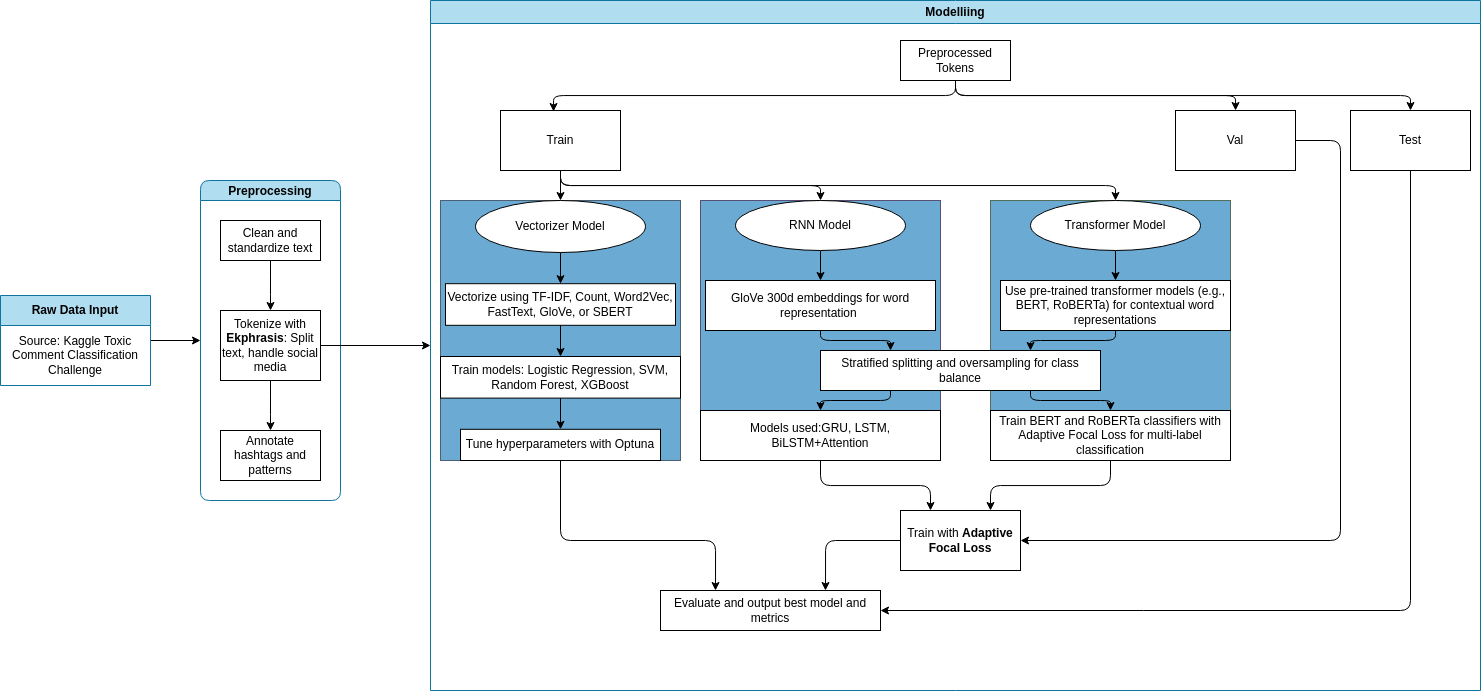
\includegraphics[width=0.3\textwidth]{figures/flowchat.png}
            \captionof{figure}{Overview of the model pipeline for toxic comment classification}
            \label{fig:model_pipeline}
        \end{center}
        }

